\documentclass[12pt,a4paper,oneside]{article}
\usepackage{graphicx,setspace,float,fancyhdr,listings,xcolor,placeins,xeCJK,tocloft}
\setCJKmainfont[AutoFakeBold=3]{STFangsong} % CJK Font Setup
\usepackage[dvipsnames]{xcolor}
\renewcommand{\cftsecleader}{\cftdotfill{\cftdotsep}} % Enable dot leaders
\renewcommand{\cftdotsep}{1} % Adjust dot spacing (1 is for close dots; increase for more spacing)
\setcounter{tocdepth}{3} % Set table of contents depth
\setstretch{1.25}


% 设置页眉和页脚
\setlength{\headheight}{13.6pt} % 设置页眉高度
\addtolength{\topmargin}{-1.6pt} % 调整上边距
\pagestyle{fancy}
\fancyhf{}
\fancyhead[C]{\small Python} % 中间页眉
\fancyfoot[C]{\small \thepage} % 中间页脚
\author{}
% 设置代码高亮样式
\lstset{
    language=Python,                 % 代码语言
    title=\lstname,                  % 标题显示代码文件名
    captionpos=b,                    % 标题位置(b表示底部)
    % 基本样式
    basicstyle=\ttfamily\small,      % 代码字体样式和大小
    keywordstyle=\bfseries\color{NavyBlue}, % 关键字样式
    commentstyle=\itshape\color{red!50!green!50!blue!50}, % 注释样式
    stringstyle=\bfseries\color{PineGreen!90!black}, % 字符串样式
    emph={self},                     % 指定强调词
    emphstyle=\bfseries\color{Rhodamine}, % 强调词样式
    % 背景与框架设置
    backgroundcolor=\color{black!3}, % 背景色
    frame=shadowbox,                 % 框架样式(阴影框)
    frameround=fttt,                 % 圆角样式
    rulesepcolor=\color{red!20!green!20!blue!20}, % 阴影框的颜色
    rulecolor=\color{black},         % 框架线颜色
    % 行号设置
    numbers=left,                    % 行号位置
    numberstyle=\tiny,               % 行号字体样式
    stepnumber=1,                    % 行号间隔
    numbersep=5pt,                   % 行号与代码间距
    % 布局设置
    showspaces=false,                % 是否显示空格
    showstringspaces=false,          % 是否显示字符串中的空格
    showtabs=false,                  % 是否显示制表符
    tabsize=4,                       % 制表符宽度
    breaklines=true,                 % 自动换行
    breakatwhitespace=false,         % 仅在空格处换行(false则不限定)
    columns=flexible,                % 列样式
    % 代码块的边距与间距设置
    xleftmargin=1em,                 % 左边距
    xrightmargin=-2em,               % 右边距
    aboveskip=1em,                   % 代码块上方的间距
    framexleftmargin=2em,            % 阴影框左边距
    % 其他设置
    escapeinside=``,                 % 允许在代码块中使用 LaTeX 命令
    morekeywords={}                  % 自定义更多关键字
}

\title{
    \vspace*{-2cm} % 调整垂直间距,使图像顶格显示
    
\includegraphics[width=0.8\textwidth]{SYSULogo.pdf} \\[1em]
    \vfill % 添加弹性空间,使内容居中
    \LARGE \textbf{Python第二次大作业} \\[1em]
    \Large
    \begin{tabular}{rl}
        \textbf{姓名:} & \textbf{陈海弘} \\
        \textbf{学号:} & \textbf{23354049}
    \end{tabular}
    \vfill % 添加弹性空间,使内容居中
}
\date{\Large 2024.11.11}

\begin{document}

\maketitle

\newpage
\tableofcontents
\newpage
\section{摘要}
这次作业主要包括三个题目,分别是读取统计、学生成绩分析和账户注册登录系统。第一题要求读取news.txt文件中的单词,统计每个单词出现的次数,并按照字母顺序写入另一个文件。第二题要求对学生成绩数据进行分析,包括计算数学成绩的平均值、中位数、最小值和最大值,统计阅读成绩各分数段的人数并用柱状图可视化,计算每个学生的平均成绩并按照平均分从高到低进行排名,绘制不同性别的数学成绩分布箱线图,计算参加考前准备课程的学生和未参加考前准备课程的学生各科目平均成绩并制作堆积柱状图进行比较。第三题要求实现账户注册、登录和修改密码功能,并对用户输入的密码进行评分,根据评分结果输出密码强度等级。
\section{题目}
\subsection{读取统计}
题目要求:
第一题(20分)
文本文件“news.txt”中包含了一些英文单词,每个单词占据文件的一行。请编写一个Python程序,该程序读取文件并统计每个单词出现的次数,然后将单词及其出现次数按照字母顺序写入另一个文件。格式如下:
Area: 1
Bay: 1
Greater: 1

思路:
首先读取news文件内容,考虑到是每一行一个单词,所以可以直接按行读取,要统计单词出现的次数,可以创建字典,key作为单词,value作为出现次数,这样就能实现统计功能。
读取时for循环每一次读取一行,然后判断是否在字典中,如果在则value+1,否则添加到字典中。
然后对字典按照key进行排序,然后写入文件。排序的时候要用lambda函数判断key首个字母的大小写,这样就能实现字母顺序排序。最后写入文件即可。

重要代码:
\begin{lstlisting}
    with open("news.txt", "r") as f:
    for line in f:  # 按行读取
        word = line.strip()
        wordTotal[word] = wordTotal.get(word,0) + 1 # 统计单词出现次数,如果单词不存在则默认为0
sortedwords = sorted(wordTotal.keys(), key = lambda x: (x[0].islower(),x))  # 按照字母顺序排序,lambda函数用于排序时区分大小写
\end{lstlisting}

\begin{figure}[H]
    \centering
    \begin{minipage}{0.1874\textwidth}
        \centering
        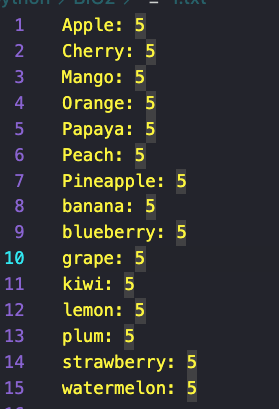
\includegraphics[width=\textwidth]{image/1} % 替换为你的图片文件名
        \caption{结果}
        \label{fig:image1}
    \end{minipage}
\end{figure}


\subsection{学生成绩分析}
题目要求:第二题(35分)
现有一个包含学生考试成绩数据的CSV文件,包括以下列:Gender(性别)、Test Preparation Course(是否参加考前准备课程)、Math(数学成绩)、Reading(阅读成绩)、Writing(写作成绩)。

请利用Numpy、Matplotlib等工具对数据进行分析,回答下列问题:

1、 计算数学成绩的平均值、中位数、最小值和最大值。

2、 统计阅读成绩各分数段的人数(每10分为一段),并用柱状图可视化它们的分布。

3、 计算每个的学生的平均成绩,并按照平均分从高到低进行排名,并制作一个水平条形图展示排名结果(可使用编号表示人员信息)。

4、 根据性别,绘制一个箱线图,显示不同性别的数学成绩分布。

5、 计算参加考前准备课程的学生和未参加考前准备课程的学生各科目平均成绩,并制作一个堆积柱状图进行比较。

思路:

1.读取文件后,用np中的mean,median,min,max函数计算数学成绩的平均值、中位数、最小值和最大值。

2.分数段统计,观察数据的最大值和最小值在60到110之间,创建bins,间隔为10,然后用cut函数将数据分段,再用value\_counts函数统计各分数段的人数,最后用bar函数绘制柱状图。这里要注意对数据按照索引排序。最后用plt.plot()显示图像。

3.使用mean(axis=1)计算每位学生的三科平均分,并将结果保存到Average Score列。按Average Score降序排序,并绘制水平条形图展示学生的平均成绩排名。

4.使用boxplot,通过Gender分组绘制数学成绩的箱线图,以便比较性别之间的数学成绩分布。

5.按Test Preparation Course分组,计算数学、阅读和写作三科的平均分。
通过stacked=True绘制堆积柱状图,比较不同课程准备情况的平均成绩差异。

重要代码及实现:
1.
\begin{lstlisting}
    mathScore = data['Math']
    mathMean = np.mean(mathScore)
    mathMidian = np.median(mathScore)
    athMin = np.min(mathScore)
    mathMax = np.max(mathScore)
\end{lstlisting}

\begin{figure}[H]
    \centering
    \begin{minipage}{0.6\textwidth}
        \centering
        
\includegraphics[width=\textwidth]{image/Figure_0} % 替换为你的图片文件名
        \caption{结果}
        \label{fig:image2}
    \end{minipage}
\end{figure}

2.\begin{lstlisting}
    bins = range(60, 110, 10)   # 60-70, 70-80, 80-90, 90-100
    reading_score_counts = pd.cut(data['Reading'], bins=bins).value_counts().sort_index()   #cut函数,将数据进行分段,value_counts()统计每个分段的个数,sort_index()按索引排序
\end{lstlisting}

\begin{figure}[H]
    \centering
    \begin{minipage}{0.4\textwidth}
        \centering
        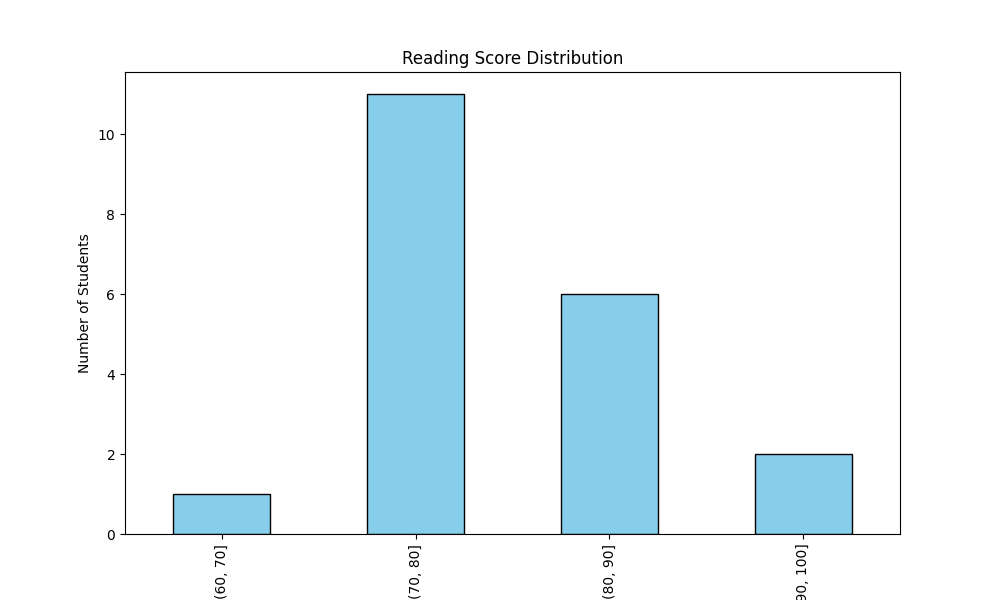
\includegraphics[width=\textwidth]{image/Figure_1.png} % 替换为你的图片文件名
        \caption{结果}
        \label{fig:image3}
    \end{minipage}
\end{figure}

如图~\ref{fig:image3}所示,统计阅读成绩的各分数段的人数并用柱状图可视化,可以看出阅读成绩主要集中在70-80分段。


3.\begin{lstlisting}
    data['Average Score'] = data[['Math', 'Reading', 'Writing']].mean(axis=1)   #data[['Math', 'Reading', 'Writing']]选取三科成绩列,mean(axis=1)计算每行的平均值
    data_sorted = data.sort_values(by='Average Score', ascending=False)  #sort_values(by='Average Score', ascending=False)按平均成绩降序排列
\end{lstlisting}

\begin{figure}[H]
    \centering
    \begin{minipage}{0.4\textwidth}
        \centering
        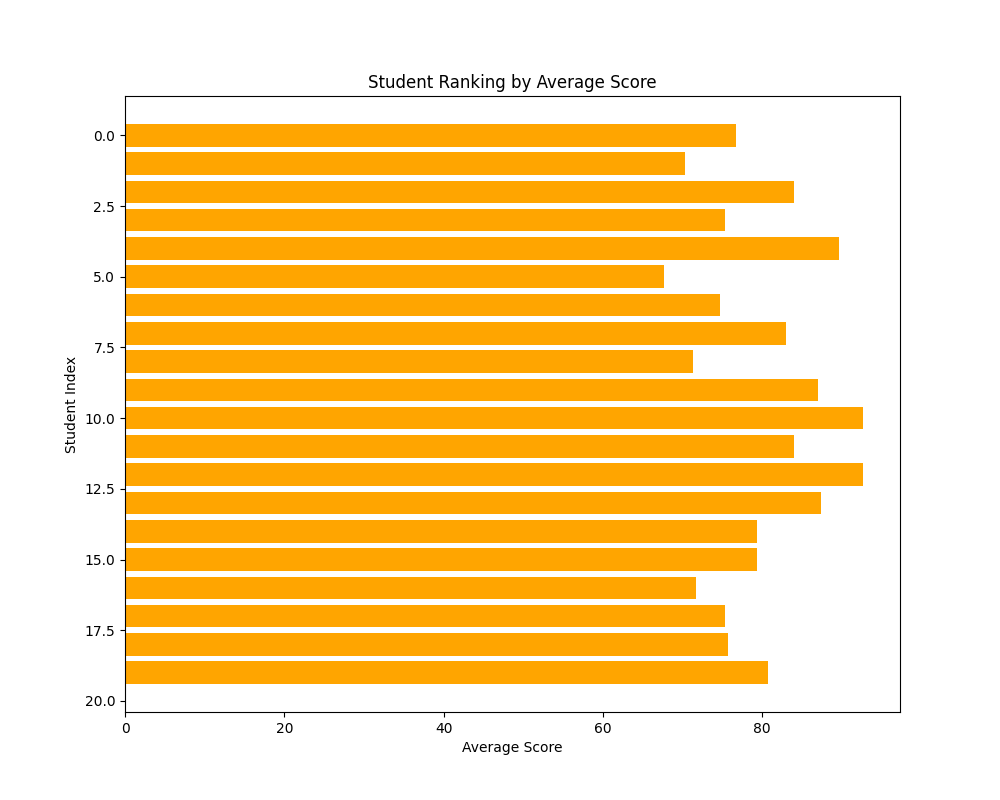
\includegraphics[width=\textwidth]{image/Figure_2.png} % 替换为你的图片文件名
        \caption{结果}
        \label{fig:image4}
    \end{minipage}
\end{figure}

如图~\ref{fig:image4}所示,绘制了学生的平均成绩排名水平条形图,可以看出学生的平均成绩从高到低依次为学生编号4、5、6、7、8、9、10、1、2、3。

4.\begin{lstlisting}
    plt.figure(figsize=(8, 6))
    data.boxplot(column='Math', by='Gender', grid=False)    #by是根据性别分组,grid=False去掉网格线,column='Math'表示绘制数学成绩的箱线图
\end{lstlisting}

\begin{figure}[H]
    \centering
    \begin{minipage}{0.4\textwidth}
        \centering
        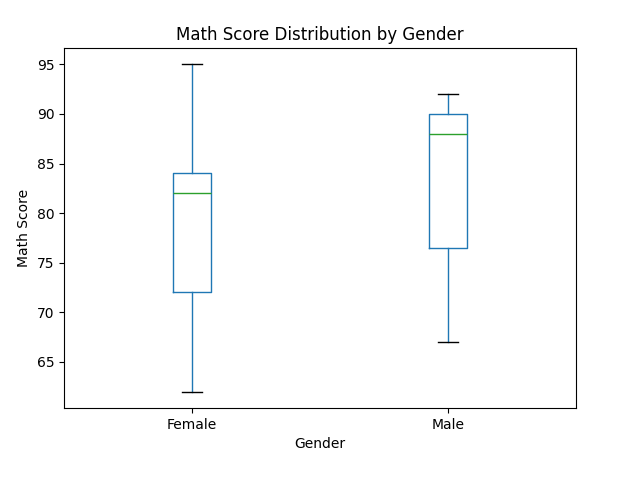
\includegraphics[width=\textwidth]{image/Figure_3.png} % 替换为你的图片文件名
        \caption{结果}
        \label{fig:image5}
    \end{minipage}
\end{figure}


如图~\ref{fig:image5}所示,绘制了不同性别的数学成绩分布箱线图,可以看出女生的数学成绩中位数略高于男生。


5.\begin{lstlisting}
    course_group = data.groupby('Test Preparation Course')[['Math', 'Reading', 'Writing']].mean()
    course_group.plot(kind='bar', stacked=True, color=['lightcoral', 'skyblue', 'lightgreen'], edgecolor='black', figsize=(10, 6))  #stacked=True绘制堆积柱状图,color设置颜色,edgecolor='black'设置边框颜色
\end{lstlisting}

\begin{figure}[H]
    \centering
    \begin{minipage}{0.4\textwidth}
        \centering
        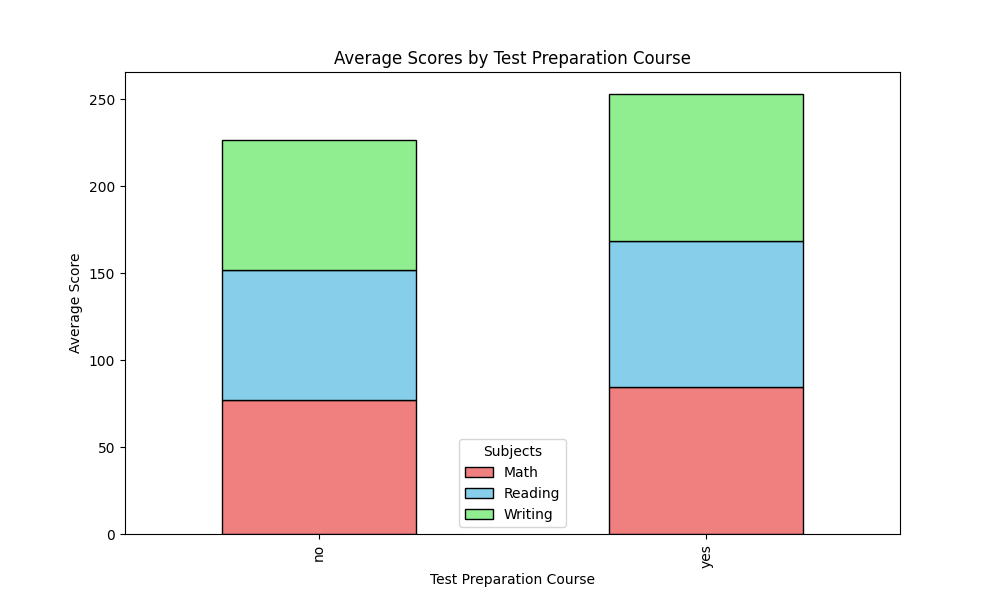
\includegraphics[width=\textwidth]{image/Figure_4.png} % 替换为你的图片文件名
        \caption{结果}
        \label{fig:image6}
    \end{minipage}
\end{figure}


如图~\ref{fig:image6}所示,绘制了参加考前准备课程的学生和未参加考前准备课程的学生各科目平均成绩的堆积柱状图,可以看出参加考前准备课程的学生在数学、阅读和写作三科的平均成绩均高于未参加考前准备课程的学生。
\subsection{账户注册登录系统}
题目要求:


用Python编写程序,进行账户(保存的账户信息包括姓名、学号和密码评分)的注册和登陆,并对于用户输入的密码进行评分。
实现功能:1.程序启动后,可选择三种操作注册,登陆,修改密码。2.注册要求用户输入新用户名和密码,同时进行密码评分,要进行用户名重复性检验,不能与已有用户名重复,注册成功后要录入账户信息,输入姓名(可不与用户名相同),学号。3.登录需要输入正确的用户名及密码,登陆成功后打印账户中保存的信息。4.修改密码要求先输入原密码再输入新密码,同时进行密码评分,若原密码错误则不可修改。5.可以适当完善修改账户信息的功能(选做)。
要求至少实现三名用户的信息保存,需测试注册,登陆,修改密码等功能,并验证保存账户的有效性。
 
密码按如下规则进行计分(累计),规则如下:

一、密码长度:
5 分: 小于等于4 个字符
10 分: 5 到7 字符
25 分: 大于等于8 个字符

二、字母:
0 分: 没有字母
10 分: 全都是小(大)写字母
20 分: 大小写混合字母

三、数字:
0 分: 没有数字
10 分: 1 个数字
20 分: 大于1 个数字

四、符号:
0 分: 没有符号
10 分: 1 个符号
25 分: 大于1 个符号

五、奖励:
2 分: 字母和数字
3 分: 字母、数字和符号
5 分: 大小写字母、数字和符号
 
在获得一个密码后,根据如下的评分规则:
>= 90: 非常安全
>= 80: 安全
>= 70: 非常强
>= 60: 强
>= 50: 一般
>= 25: 弱
>= 0:  非常弱
并输出最终的评估结果
 
密码等级样例:
38\$@NoNoNo     期望输出:您的密码属于非常安全等级
123    期望输出:您的密码属于弱等级
 

\textbf{思路}:
\begin{itemize}
    \item 首先定义一个`Account`类,用于存储账户信息。包含姓名、学号、用户名、密码等属性。
    \item 接着在程序中,通过定义密码评分函数来对用户输入的密码进行强度评估。密码评分的依据包括密码的长度、字母(大小写)、数字以及特殊符号的数量。密码的评分通过正则表达式匹配来实现,对于每个密码特征进行加分,最终得到一个总分数。基于这个分数,系统将密码的强度评定为“非常安全”、“安全”、“强”、“一般”、“弱”或“非常弱”。
    \item 然后,程序实现了用户注册、登录和修改密码功能:

	1.	注册功能:用户输入用户名、密码、姓名和学号,系统根据密码评分返回密码的强度并存储账户信息。
	
    2.	登录功能:用户输入用户名和密码进行验证,如果匹配则登录成功并显示账户信息。
	
    3.	修改密码功能:用户输入当前密码验证后,允许更改密码,并对新密码进行评分和评定强度。

\end{itemize}

\textbf{重要代码}:
\begin{lstlisting}
    # 字母评分
    if re.search("[a-z A-Z]", password): # re.search()用于在字符串中查找匹配项
        if re.search("[a-z]", password) and re.search("[A-Z]", password):   # 包含大小写字母
            score += 20
        else:
            score += 10

    # 数字评分
    digit_count = len(re.findall("[0-9]", password))
    if digit_count == 1:
        score += 10
    elif digit_count > 1:
        score += 20

    # 符号评分
    symbol_count = len(re.findall("[^a-z A-Z 0-9]", password))    # ^表示非
    if symbol_count == 1:
        score += 10
    elif symbol_count > 1:
        score += 25

    # 奖励评分
    if re.search("[a-z A-Z]", password) and re.search("[0-9]", password):
        if symbol_count > 0 and re.search("[a-z]", password) and re.search("[A-Z]", password):
            score += 5
        elif symbol_count > 0:
            score += 3
        else:
            score += 2

    return score
    # 注册新用户
    def register():
        username = input("请输入用户名: ")
        if any(acc.username == username for acc in accounts):
            print("用户名已存在,请选择其他用户名。")
            return
    
        password = input("请输入密码: ")
        score = score_password(password)
        print(f"密码评分为 {score},属于 {evaluate_password_strength(score)} 等级。")
    
        name = input("请输入姓名: ")
        student_id = input("请输入学号: ")
        new_account = Account(username, name, student_id, score)
        new_account.password = password
        accounts.append(new_account)
        print("注册成功!")
    
    # 用户登录
    def login():
        username = input("请输入用户名: ")
        password = input("请输入密码: ")
        account = next((acc for acc in accounts if acc.username == username and acc.password == password), None)
        
        if account:
            print("登录成功!")
            print(f"用户名: {account.username}, 姓名: {account.name}, 学号: {account.student_id}, 密码评分: {account.password_score}")
        else:
            print("用户名或密码错误。")
    
    # 修改密码
    def change_password():
        username = input("请输入用户名: ")
        old_password = input("请输入原密码: ")
        account = next((acc for acc in accounts if acc.username == username and acc.password == old_password), None)
        
        if account:
            new_password = input("请输入新密码: ")
            score = score_password(new_password)
            print(f"新密码评分为 {score},属于 {evaluate_password_strength(score)} 等级。")
            
            account.password = new_password
            account.password_score = score
            print("密码修改成功!")
        else:
            print("用户名或原密码错误,无法修改密码。")
\end{lstlisting}

\newpage
功能实现:
\begin{figure}[H]
    \centering
    \begin{minipage}{0.4\textwidth}
        \centering
        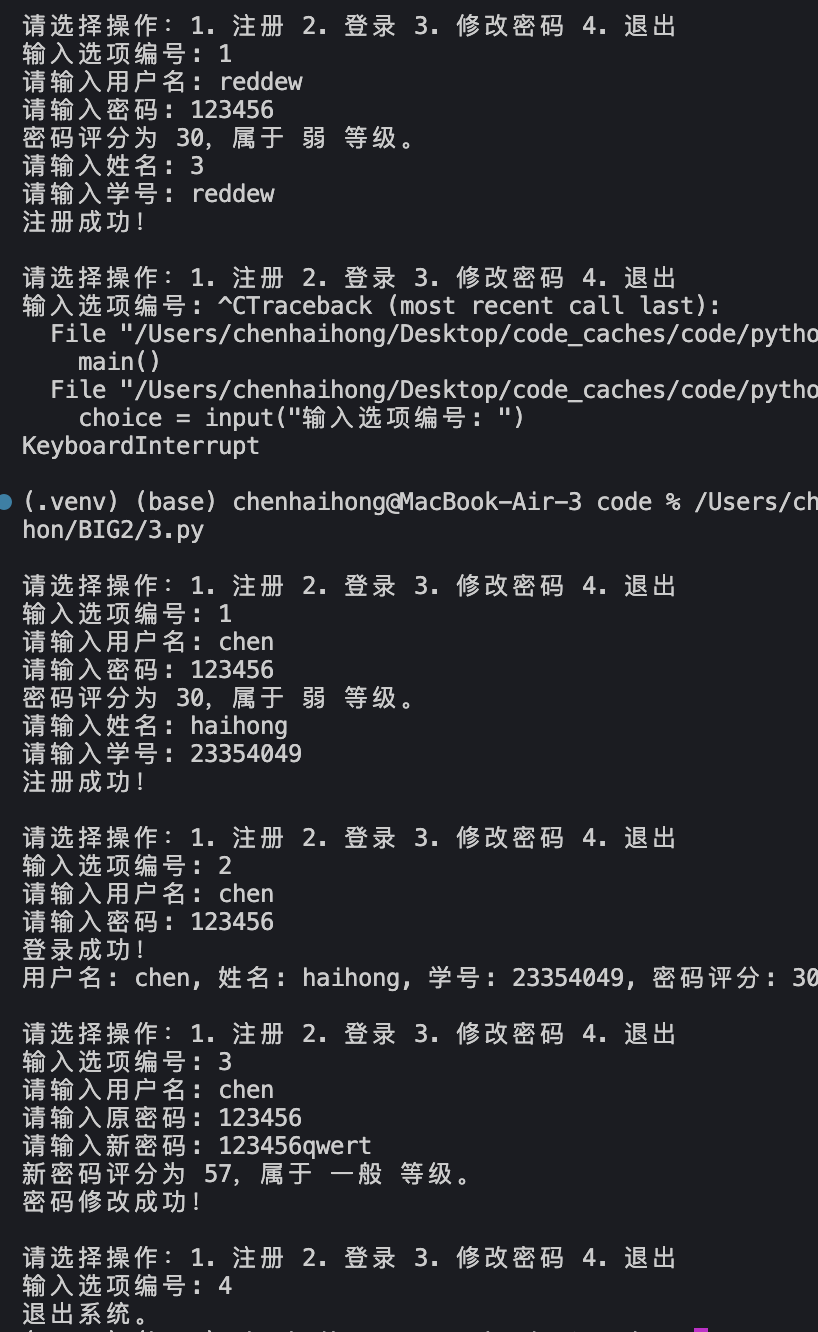
\includegraphics[width=\textwidth]{image/2} % 替换为你的图片文件名
        \caption{结果}
        \label{fig:image7}
    \end{minipage}
\end{figure}

如图~\ref{fig:image7}所示,程序实现了账户注册、登录和修改密码功能,用户可以根据提示输入用户名、密码、姓名和学号,系统会根据密码评分返回密码的强度并存储账户信息。用户登录时,输入用户名和密码进行验证,如果匹配则登录成功并显示账户信息。修改密码时,用户输入当前密码验证后,允许更改密码,并对新密码进行评分和评定强度。

\newpage
\section{总结}
这次作业总结,简单讲讲每部分的内容和遇到的一些难点吧:

	1.	文件读取与统计
要求我们写一个Python程序,从news.txt文件里读取所有单词,然后统计它们的出现次数并按字母顺序保存到新文件里。这看似简单,其实涉及到几个小难点,比如:
	
•	如何快速过滤掉标点符号和大小写,确保统计干净的单词。

•	写入文件时排序的实现,用字典来记录每个单词的次数是常规做法,但要按字母顺序输出需要额外的排序操作。

2.	学生成绩分析

用到Numpy和Matplotlib来分析学生成绩的CSV文件,这是数据处理和可视化的练手项目,内容有点多:

•	计算数学成绩的均值、中位数等统计指标是基础,不过要确保代码逻辑的严谨性。

•	阅读成绩的分布用柱状图可视化,这要求对数据的理解比较透彻,才能决定图表类型。

•	对每个学生的总成绩排名和性别的成绩差异分析,这些涉及对数据的分组和比较,写代码实现这些操作可能稍复杂。

•	最后,考察课程效果的堆积图,需要从原始数据中提取并进行数据汇总,难点在于处理数据分类和正确绘图。

3.	账户系统

这个任务包括了注册、登录、修改密码的功能,看似是个小项目,但有几个细节上要小心:


•	注册时要检查用户名是否重复,这里可以用字典或文件保存用户信息。

•	密码修改要求验证原密码是否正确,这部分涉及到密码存储和比对。

•	用正则表达式评估密码强度是一个难点,得写好规则来评估长度、字母种类、数字数量和符号,这部分对正则表达式的理解要求较高。


每部分都有自己的“坑”,这次练习下来基本涵盖了数据处理、文件操作、简单数据分析、绘图和基础正则表达式的实战。对于Python中numpy、pandas、matplotlib等库的使用我有了更深入的了解,也对数据处理和可视化有了更多的实践经验。
\end{document}